%\subsubsection*{State of the art}

\subsubsection*{Positron electron tomography:}

A PET (Positron-Electron Tomography) is a functional scan ---it does not show anatomic features--- whose main application is tumor diagnosis. It is based in the used of positron emitters radio-pharmaceuticals such as the fluorodeoxyglucose (FDG). Such radiotracers 
are injected into the patient prior to the scan. The emitted positrons slow down in the surrounding patient’s tissue, annihilating with atomic electrons to give two back-to-back 511 keV annihilation photons. The annihilation occurs within a few millimetres from the positron source. By detecting the two photons in coincidence and the coordinates of their interaction points in a detector, it is possible to define a line of response (LOR) along which the positron emitting source is located in the patient. A set of such intersecting lines allows 3D reconstruction of the source. 

%The main requirements for a PET detector are: (a) high photon detection efficiency ($\sim$ 80\% for each 511 keV gamma), (b) position resolution of a few millimetres, (c) time resolution to reduce the rate of false coincidences, (d) good energy resolution (20\% FWHM is typical in many commercial devices) to discriminate photons scattered in the patient and (e) a high count rate capability ($\sim10^6$~ s$^{-1}$ per cm$^2$~ of detecting surface). In addition, a PET system must have an angular acceptance as large as possible, which in turn requires a large axial (along the patient's body) coverage. However, due to the high cost of this devices, the axial size of a PET is typically limited to 15-20 cm. 

\subsubsection*{LYSO crystals:}

\begin{figure}[!htb]
	\centering
	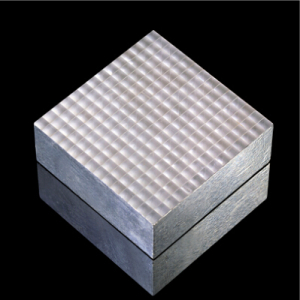
\includegraphics[scale=0.5]{img/LysoSegmented.png}
	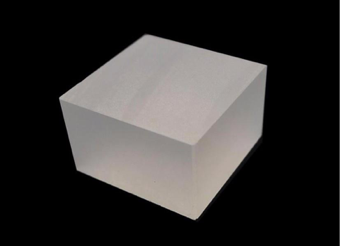
\includegraphics[scale=0.6]{img/LysoMono.png}
	\caption{\label{fig.lyso} LYSO crystals. Left: segmented; right: monolithic.  }
\end{figure}

Most of today's top-of-the-line PET scanners are based in  Lutetium oxyorthosilicate (LSO) or  
Lutetium Ytrium oxyorthosilicate (LYSO) crystals, readout by light sensitive detectors (the field is swiftly replacing photomultipliers by  SiPMs). The crystals, in turn, can be segmented (figure \ref{fig.lyso}--left), forming a matrix
of small pixels (typically $3\times 3 \times 24 \mathrm{mm^3}$), where each pixel is readout by one SIPM, or monolithic (figure \ref{fig.lyso}--right), that is, a single block readout by a matrix of SiPMs, which views the whole crystal. LYSO detectors
are characterised by: a) high density ($\rho_{LYSO} =7.4~\mathrm{g/cm^3}$) and small attenuation length 
($\lambda_{LYSO} =12$~mm for gammas of 511 keV), which permits very compact devices; b) large photon yield
($Y_{LYSO} =14000$~photons for a 511 keV gamma) which result in good energy resolution 
$\sigma^E_{LYSO} \sim12-15$~\% FWHM, for 511 keV gammas); a fast decay scintillation decay constant
($\tau_{LYSO} = 40$~ns), which permits good Coincidence Resolving Time (CRT), essential for TOF applications. 

To achieve good spatial resolution LYSO crystals are finely instrumented. For example, a segmented detector of pixel size $3 \times 3 ~\mathrm{mm^2}$~achieves a rms resolution $\sim \mathrm{3 mm/\sqrt{12} = 0.87~ mm}$~(2 mm FWHM). The resolution in the depth of interaction (DOI) of segmented detectors, on the other hand, is mediocre. For example, a crystal of 20 mm thickness, achieves a DOI resolution of  
$\sim \mathrm{20 mm/\sqrt{12} = 5.8~ mm}$~rms or about 13 mm FWHM. Monolithic detectors used the pattern information recorded by the SiPM matrix to infer the three spatial coordinates, improving the DOI resolution to some 5 mm. 

\subsubsection*{Sources of noise in a PET scanner and TOF measurements}

The reconstruction of the image in a PET system requires crossing many LORs which in turn define one emission point in the area under study. A LOR can be formed by: 1) a {\bf true coincidence}, which occur when both photons from an annihilation event are detected, neither photon undergoes any form of interaction prior to detection, and no other event is detected within the coincidence time-window; 2)
a {\bf scattered coincidence}, which occurs when one or both detected photons undergo at least one Compton scattering interaction prior to detection;
%Since the direction of the photon changes due to the scattering process, the resulting coincidence event will, most likely, produce a wrong LOR. Scattered coincidences add a background to the true coincidence distribution, decreasing contrast and causing the isotope concentrations to be overestimated. They also add statistical noise to the signal; 
3)  a {\bf random coincidence}, which occurs when two photons, not arising from the same annihilation event, impinge the detectors within the coincidence time window of the system. Both scattered and random coincidences  add statistical noise to the data. 

\paragraph{Photon detection sensitivity}

The sensitivity, $S$~ of a PET scanner represents the relationship between the recorded true coincidences and the true activity of a positron-emitting source. The two principal elements influencing the sensitivity are the scintillation crystal’s efficiency and scanner geometry. The efficiency of the scintillator material is mainly dependent on its density, atomic number, and thickness, whereas the most important geometric component of scanner is the active detection area. For a point source located in the center of a cylindrical scanner of diameter $D$~and axial length $L$, the sensitivity 
can be simply expressed as:
%
\begin{equation}
S = \frac{L}{D} \cdot \epsilon^2 \cdot \xi
\label{eq.sensi}
\end{equation}
%
where $\epsilon$~is the individual crystal (or detection cell) efficiency, and $\xi$~ measures the absorption of the gammas in the crystal (cell), $\xi = e^{-\mu \cdot t}$, where $\mu$~is the linear attenuation coefficient of 511 keV photons in the detector material and $t$~is the crystal (cell) thickness. Note that the factor $\epsilon^2$~comes from the need to form a coincidence with two crystals (cells) with efficiency $\epsilon$. Assuming that the scanner crystals 

Notice that $S$~depends linearly of the axial length ($L$) and absorption ($\xi$) but quadratically of the efficiency, due to the need to form a coincidence with two crystals (cells) with efficiency $\epsilon$. 

\subsubsection*{TOF PET}

\begin{figure}[!htb]
	\centering
	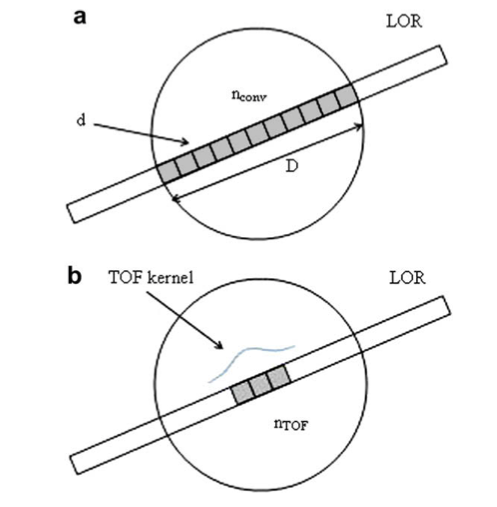
\includegraphics[scale=0.8]{img/TOF.png}
	\caption{\label{fig.tof} (a) In conventional PET reconstruction, all volume elements $n$~ found in the object along the line of response contribute to the noise in each image element, and $n_{conv} = D/d$. (b) In PET--TOF reconstruction, because of the better localisation of each event along the LOR, only the volume elements $n$~ adjacent to the position identified by the measured TOF contribute to the local noise, and $n_{TOF} = \Delta x/d$. The time resolution  $\Delta t$ limits the number of elements contributing to the noise, since it determines the localisation uncertainty $\Delta x$. }
\end{figure}


Time-of-flight (TOF) information is {\em always} used in a PET scanner to determine if two detected photons are in ``time coincidence'' and therefore belong to the same positron annihilation event.
Each detected photon is tagged with a detector position and detection time: if the detection time difference between two photons is smaller than a pre-set coincidence window (typically of the order of a few ns), the two events are considered physically correlated to the same annihilation event. 

Conventional PET reconstruction uses the TOF information only to identify the line along which the annihilation occurred. It is unable, though, to determine which voxel along the line is the source of the two photons; therefore all the voxels along the line are given the same probability of emission (figure \ref{fig.tof}--a). PET--TOF uses the time-of-flight difference to better locate the annihilation position of the emitted positron. The time-of-flight  difference $\Delta t$~ is directly related to the distance $x$~ of the annihilation point from the center of the field of view (FOV), $x = c \Delta t/2$, along the LOR identified by the two detectors in coincidence. The limiting factor to localise the annihilation point is the uncertainty in the measured time difference $\delta \Delta t$, or CRT (Coincidence Resolving Time) of the system. The time resolution is used in the reconstruction algorithm as a kernel for a localisation probability function, as shown in figure \ref{fig.tof}--b. It can be shown that TOF reconstruction is equivalent to an amplification of the PET scanner sensitivity, according to:
%
\begin{equation}
S_{tof} = \frac{D}{\delta x} S_{conv}
\label{eq.sensiTOF}
\end{equation}
%
where $S_{tof}$~is the sensitivity of a PET-TOF system, $S_{conv}$~is the sensitivity of a conventional scanner, 
$D$~is the diameter of the object being imaged and $\delta x = c \delta \Delta t/2 \propto CRT$, 
thus, $S_{tof} \propto \frac{D}{CRT} S_{conv}$. It follows that the gain in sensitivity is directly proportional to the size of the patient and inversely proportional to the CRT. In other words, large patients will particularly benefit from TOF reconstruction.

Currently there is a commercial system based in LYSO crystals, the GEMINI of Philips\footcite{GEMINI}, capable to reach a CRT of 600 ps. Laboratory setups with LYSO crystals reach values in the range of 150--300 ps, depending on the experimental conditions. For example Ferri et al\footcite{LysoFBK}
 report measurements using a pair of small LYSO crystals 
($3 \times 3 \times 5 {\rm mm^3}$) readout by high-fill factor SiPMs. With this setup, a CRT of $157\pm 5$~ ps was found at ambient temperature.

\subsubsection*{Physical properties of liquid xenon relevant for PET}

Xenon is a noble gas. It responds to the interaction of ionizing radiation producing about 60 photons per keV of deposited energy. The emitted photons have wavelengths in the ultraviolet range (VUV)
with an average wavelength of 178 nm. The scintillation signal is fast 
(see below) and can thus result in an excellent CRT.  In its liquid phase (at a temperature of $\sim$ 160 K and atmospheric pressure) LXe has a reasonable high density (3 g/cm$^3$) and an acceptable attenuation length (36 mm), which makes it suitable for PET applications. Its main attractive features are:

\begin{enumerate}
\item {\bf A high scintillation yield (30,000 photons per 511 keV gamma)}, twice as large as that of LYSO. 
\item {\bf LXe is a continuous medium with uniform response}. The design of a compact system is much simpler, then, than when using solid detectors of fixed shape. It is also possible to provide a 3D measurement of the interaction point, and, thus, a high resolution measurement of the DOI. Furthermore, in LXe it is possible to identify Compton events depositing all its energy in the detector as separate-site interaction, due to its relatively large interaction length. This increases the sensitivity of the system, since those events can, in principle, be used for image reconstruction. 
\item {\bf The temperature of LXe at atmospheric pressure (160 K or -113 C)} is hot enough as to permit a simple cryostat, as well as normal operation of the SiPMs, but cold enough to reduce the dark current rate (DCR) of the SiPMs by a factor $\sim 2^{13}$, thus making it essentially negligible. 
\item {The cost} of LXe is 3 \euro/cc to be compared with $\sim$ 40-50 \euro/cc in the case of LYSO. 
 \end{enumerate}

%The first idea of using a LXe time projection chamber for PET was proposed in 1993 by Chepel \cite{chepelFirst}. 
The possibility of building a LXe PET based on the excellent properties of LXe as scintillator was first suggested by Lavoie in 1976  \footcite{lavoie}, and the study of this type of PET was carried out by the Waseda group \footcite{Doke1,Nishikido2,Nishikido1}. 

\subsubsection*{PETALO}


\begin{figure}[!htbp]
	\centering
	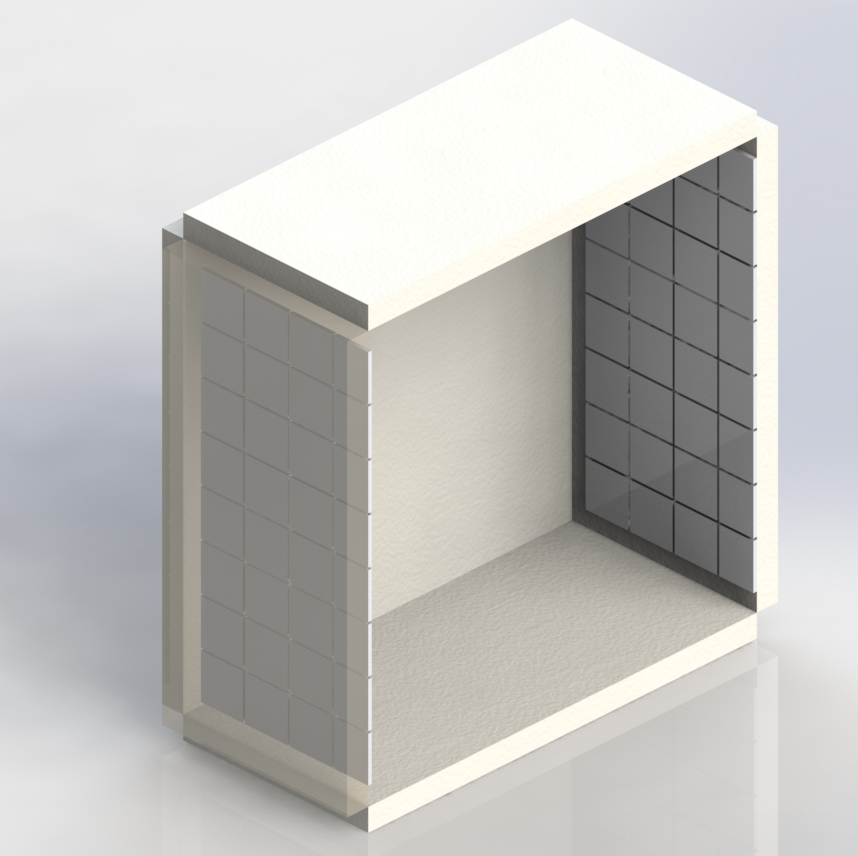
\includegraphics[scale=0.20]{img/Box_2faces_1.jpg}
	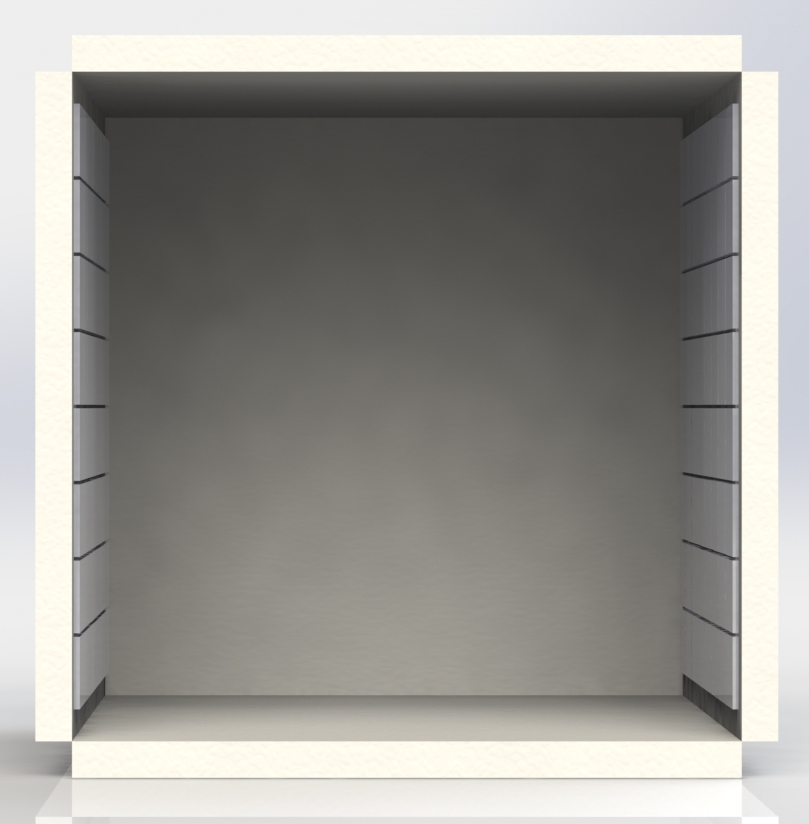
\includegraphics[scale=0.20]{img/Box_2faces_3.jpg}
	\caption{The LXSC2 instruments the entry and exit faces of the box (relative to the photon line of flight) with silicon photomultipliers (SiPMs), which can be eventually coated with TPB. The non-instrumented faces are covered by reflecting Teflon (optionally also coated with TPB).}\label{fig.box} 
\end{figure}
%\begin{figure}[!htbp]
%	\centering
%	\includegraphics[scale=0.6]{../img/LXSC2.pdf}
%	\caption{The LXSC2 instruments the entry and exit faces of the box (relative to the photon line of flight) with silicon photomultipliers (SiPMs), which can be eventually coated with TPB. The non-instrumented faces are covered by reflecting Teflon (optionally also coated with TPB).}\label{fig.box} 
%\end{figure}

PETALO (Positron Electron TOF Apparatus using Liquid xenOn) is a proposed new type of PET scanner which exploits the copious scintillation of liquid xenon and the availability of state-of-the-art SiPMs and fast electronics designed to maximise TOF performance \footcite{Petalo2015}. The detector building block is the liquid xenon scintillating cell (LXSC). The cell shape and dimensions can be optimised depending on the intended application. In particular, the LXSC2 instruments the entry and exit faces of the box (relative to the gammas line of flight) with silicon photomultipliers, while all the other faces are covered with a reflecting material such as Teflon. The SiPMs are read out by ASICs optimised for excellent timing resolution. 
 %PETALO is a compact, homogenous and highly efficient detector which shares many of the desirable properties of monolithic crystals, with the added advantage of high yield and fast scintillation offered by liquid xenon, low noise due to cryogenic operations which virtually eliminates the SiPMs DCR, and the potential of low cost. 
%

The energy resolution and spatial resolution of the LXSC2 instrumented with 6 mm SiPMs was studied in \footcite{Petalo2015}. The energy resolution was found to be 12\% FWHM for 511 keV gammas. The spatial resolution in the three coordinates was found to be 2 mm FWHM. Bot the energy resolution and the spatial resolution in the (x,y) coordinates (transverse to the gammas line of flight) were of the same order than that obtained by top of the line LYSO scanners. The resolution in the longitudinal coordinate, measuring the depth of interaction (DOI) was obtained by computing the ratio between the
total signal recorded in the instrumented entry and exit face. A DOI resolution of 2 mm is much better than that obtained by segmented LYSO crystals (unless the thickness of the crystal is very small), and compares with the best results obtained using monolithic crystals \footcite{VanDamm2011}.
%
\subsection*{VUV-sensitive SiPMs versus SiPMs coated with TPB}
%
%\begin{figure}[!htbp]
%	\centering
%	\includegraphics[scale=0.6]{../img/PDEVUV.png}
%	\caption{Photo detection efficiency (PDE) of different VUV sensitive SiPMs
%	(from http://neutrino.physics.ucdavis.edu/indico/contribAuthorDisplay.py?contribId=61\&authorId=0\&sessionId=2\&confId=17). The MEG devices are
%	manufactured by Hamamatsu Photonics, while the FBK-2010 and the RGB-HD
%	are manufactured by FBK.  }\label{fig.vuv} 
%\end{figure}
%
%\begin{figure}[!htbp]
%	\centering
%	\includegraphics[scale=0.6]{../img/TPBEfficiency.png}
%	\caption{Visible re-emission spectrum for a TPB film illuminated with 
%	128, 160, 175, and 250 nm light. All spectra are normalized to unit area.
%	(from \cite{Gehman:2011xm}).  }\label{fig.tpb} 
%\end{figure}
%
%\begin{figure}[!htbp]
%	\centering
%	\includegraphics[scale=0.6]{../img/TPBSpectrum.png}
%	\caption{Total integrated fluorescence efficiency for a thin layer of TPB, as a function of input  photon wavelength
%	(from \cite{Gehman:2011xm}).  }\label{fig.tpbeff} 
%\end{figure}
%
%\begin{figure}[!htbp]
%	\centering
%	\includegraphics[scale=0.6]{../img/PetaloTOF/TpBDecayConstant.png}
%	\caption{Evolution of the decay constant of TPB as a function of the thickness of the TPB layer compared
%	with the thickness of the substrate (a thin quartz film). The TPB decay constant decreases as the thickness of the TPB layer (thus its concentration) increases, reaching an asymptotic value of 2.2 ns.   
%	(from \cite{TPBtau}).  }\label{fig.tpbtau} 
%\end{figure}
%

The scintillation light of LXe peaks around 178 nm (VUV region). Therefore the LXSC2 needs to be instrumented either with VUV-sensitive SiPMs (as for example the upgraded LXe calorimeter of the 
MEG experiment \footcite{Ogawa:2015ucj}) or by conventional SiPMs coated with a wavelength shifter such as tetraphenyl butadiene (TPB) (as for example in the NEXT experiment \cite{Alvarez:2013gxa}). 
The VUV-SiPMs tested for the MEG as well as for the future nEXO 
experiment \cite{Ogawa:2015ucj,Ostrovskiy:2015oja} reach a PDE of about 
15\%. Further improvements of the technology could eventually result in a PDE of 20\% .  Conventional SiPMs can reach today a PDE of around 50\%.When they are coated with a thin layer of TPB, the VUV light is absorbed by the wavelength shifter with an efficiency of 80\% \footcite{Gehman:2011xm}
shifted to $\sim$ 430 nm (figure \ref{fig.tpb}) and re-emitted isotropically. The decay constant of TPB has been measured  in thin films \footcite{TPBtau} and a value of 2.2 ns is found for sufficiently large TPB concentrations. 

\subsubsection*{PETALO as a PET-TOF scanner}
The potential of PETALO as a a PET-TOF scanner has been recently studied \footcite{PetaloTOF}. The scintillation in xenon is parameterised in terms of two decay constants:

 \begin{figure}[!bhtp]
	\centering
	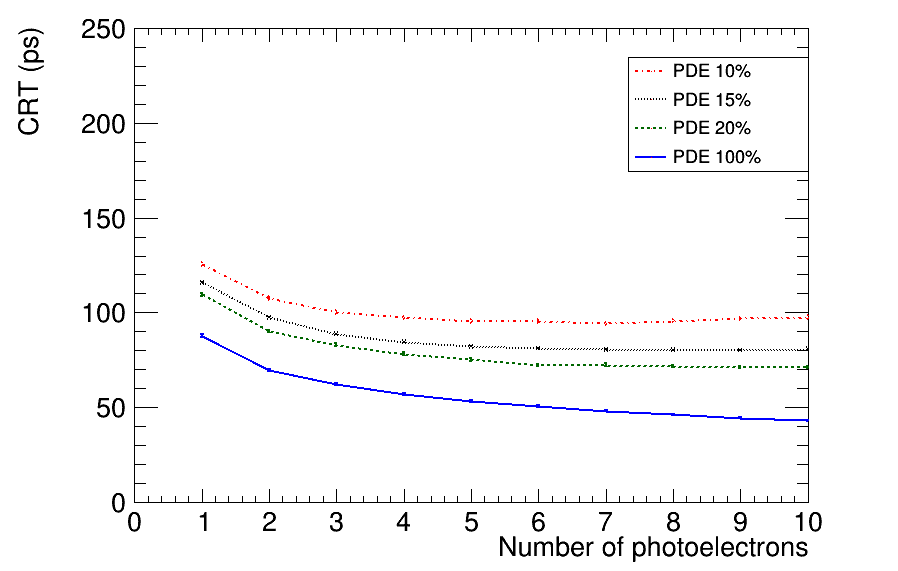
\includegraphics[scale=0.40]{img/lxe_noCher_avg_npe_phys.png}
	\caption{\label{fig.crt_avg_LXe} CRT as a function of the number of photoelectrons used to compute $\Delta t$, for LXe. The CRT is shown for several values of the PDE.}
\end{figure}

\begin{equation}
I(t) = N_\gamma (0.07 \times \frac{e^{-t/\tau_1}}{\tau_1} + 0.93 \times \frac{e^{-t/\tau_2}}{\tau_2})
\label{eq.scint}
\end{equation}
where $\tau_1 = 2.2$~ns and $\tau_2 = 27$~ns. Thus, xenon scintillation is not only more copious (by a factor two) but also much faster than scintillation in LYSO. Using VUV-sensitive SiPMs a CRT of 70 ps is found for a PDE of 20 \% (80 ps for a PDE of 15\%, see figure \ref{fig.crt_avg_LXe}). Using conventional SiPMs coated with TPB, the CRT varies between 130 and 155 ps, depending on the (poorly known) value of the TPB decay constant. This results show the
potential of the PETALO concept as a PET-TOF scanner.  

\subsubsection*{Resolving Compton interactions:}

\begin{figure}[!htbp]
	\centering
	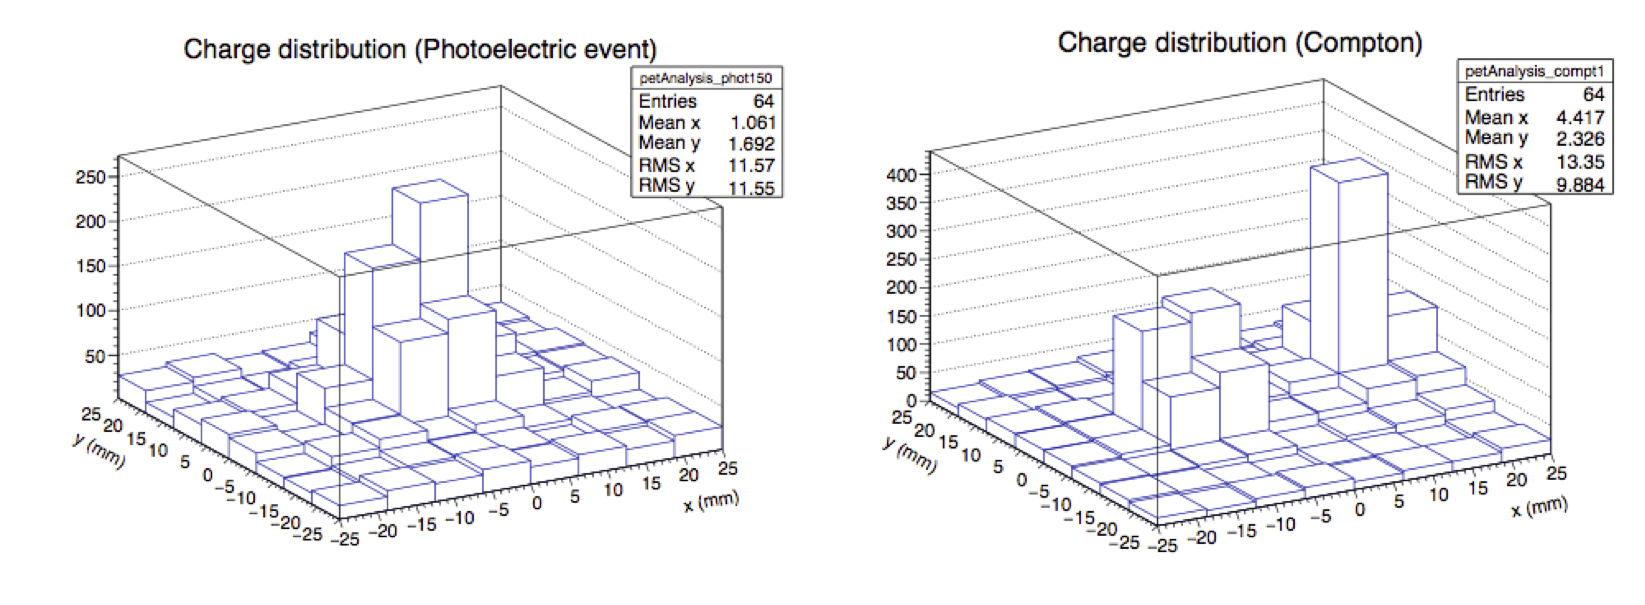
\includegraphics[scale=0.6]{img/Compton.png}
	\caption{The LXSC2 can distinguish well between 1-site photoelectric events (left panel) and
	Compton events, such as the 2-site Compton event shown in the right panel.}\label{fig.Compton} 
\end{figure}

Photoelectric interactions are a relatively small fraction of the total number of interactions in LXe (22\%) as well as in LYSO (33\%). The bulk of Compton interactions can result either in contained (when the scatter gamma produces a cascade that does not escape the detector) or non contained events. Non contained events do not deposit the full energy of the gamma in the detector and can be rejected. However, the large fraction of contained Compton events (60\% for the LXSC and larger for the denser crystals of LYSO) introduce a significant distortion of the position and contribute to the noise and to spoil the CRT. 

An important advantage of the LXSC2 is that multiple-site hits can be identified (the system measures true 3D points). Thus Compton events can either be rejected, or added to the imaging sample, in the case of 2-site interactions where each vertex is clearly identified (an example is shown in figure \ref{fig.Compton}), thus increasing sizeably the efficiency.  
%

\subsubsection*{PETALO as a Full-Body PET}
%
\begin{figure}[!htb]
	\centering
	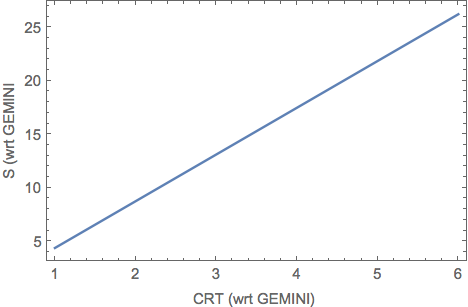
\includegraphics[scale=0.6]{img/RelativeSensitivity.png}
	\caption{\label{fig.rsensi} Relative sensitivity of a PETALO-TOF-FBP scanner w.r.t the the current top-end PET-TOF scanner, the GEMINI of Philips as a function of the relative CTR.  }
\end{figure}


A major application of the PETALO concept would be the construction of a ``Full Body PET'' (FBP), of axial dimensions in the range of 70-100 cm, exploiting the low cost and the excellent performance offered by LXe. In addition to the superb energy resolution and spatial resolution a PETALO--FBP scanner would offer a much increased sensitivity w.r.t. conventional PET devices. To illustrate this point, we combine equations \ref{eq.sensi} and \ref{eq.sensiTOF} to write the relative sensitivity of two PET scanners, $p_1,p_2$~ having the same bore and scanning a patient of the same dimensions as:

\begin{equation}
S(p_1,p_2) = \frac{L_1} {L_2}\frac{CTR_1} {CTR_2}\frac{\epsilon_1} {\epsilon_2}\frac{e^{-\mu_1 t_1}} {e^{-\mu_2 t_2}}
\label{eq.srel}
\end{equation}
%
where $L_i,CTR_i,\epsilon_1,\mu_i,t_i, i=1,2$~are the axial length, CTR, detector efficiency, linear attenuation coefficient and crystal (cell) thickness for scanners $p_1,p_2$.

We can now use equation \ref{eq.srel} to compare the performance of a 1 m axial length PETALO-TOF-FBP scanner using LXe ($\mu = 36$~mm) and based in LXSC2 cells of 50 mm thickness with the current top-end PET-TOF scanner, the GEMINI of Philips, using LYSO crystals ($\mu = 12$~mm) of 25 mm thickness. Figure \ref{fig.rsensi} shows the improvement in sensitivity as a function of the improvement in CTR, assuming that the detection efficiency of both systems is the same. A factor 10 improvement is obtained if the PETALO scanner achieves an overall CTR of 240 ps, and a factor 20 for a CTR of 130 ps, which is feasible even using cost-competitive SiPMs coated with TPB. 

The assumption that a LYSO crystal and an LXSC cell can have similar efficiencies is important and deserves some discussion. The factors that affect the efficiency are: i) the photoelectric fraction; ii) the fraction of Compton events that can be used for imaging; iii) the energy window to accept events; iv) the time window to accept events; the packing factor of the crystals (e.g, the amount of dead space between crystals needed for packing). Of this list, LYSO has a better photoelectric fraction than LXE (0.33 versus 0.2); Compton events can be better distinguished in LXe than in LYSO, allowing to increase the fraction of events useful for imaging in the LXSC2; the energy window of both system is similar, (energy resolution is of the same order); the time window in LXe is better than in LYSO (scintillation is faster); the packing in LXe is better than in LYSO, since LXe is a continuous medium and the LXSC cells can be tailored to minimise dead areas. Thus, the LXSC offers better Compton identification, time window and compactness to compensate the lower photoelectric fraction. 
%

